\documentclass[a4paper]{article}
\usepackage[UTF8]{ctex}
\usepackage{geometry}
\usepackage{graphicx}
\usepackage{url}
\usepackage{multirow}
\usepackage{array}
\usepackage{booktabs}
\usepackage{url}
\usepackage{enumitem}
\usepackage{graphicx}
\usepackage{float}
\usepackage{amssymb}
\usepackage{amsmath}
\usepackage{subfig}
\usepackage{longtable}
\usepackage{pifont}
\usepackage{color}

\allowdisplaybreaks

\geometry{a4paper, scale=0.78}

% \begin{figure}[H]
%     \centering
%     \includegraphics[width=.55\textwidth]{E.png}
%     \caption{矩阵与列向量的乘法}
%     \label{fig:my_label_1}
% \end{figure}

% \left\{
% \begin{array}{ll}
%       x+2x+z=2 & \\
%       3x+8y+z=12 & \\
%       4y+z=2
% \end{array}
% \right.

% \begin{enumerate}[itemindent = 1em, itemsep = 0.4pt, parsep=0.5pt, topsep = 0.5pt]

% \end{enumerate}

%\stackrel{a}{\longrightarrow}

%\underbrace{}_{} %下括号

%\tableofcontents %目录,并且目录页不记录页码
% \tableofcontents
% \newpage
% \setcounter{page}{1} %new page
% \clearpage

\title{Hidden Markov Model 01 Background}
\author{Chen Gong}
\date{07 January 2020}

\begin{document}
\maketitle
机器学习大致可以分为两个派别,也就是频率派和贝叶斯派的方法,这个之前,我们都有过详细的说明。这里再大致的回顾一下。

频率派的思想就衍生出了统计学习方法,说白了统计学习方法的重点在于优化,找loss function。频率派的方法可以分成三步,1. 定义Model,比如$f(w) = w^Tx+b$;2. 寻找策略strategy,也就是定义Loss function;3. 求解,也就是优化的方法,比如梯度下降(GD),随机梯度下降(SGD),牛顿法,拟牛顿法等等。

贝叶斯派的思想也就衍生出了概率图模型。概率图模型重点研究的是一个Inference的问题,我们要求的是一个后验概率分布$P(Z|X)$,其中$X$为观测变量,$Z$为隐变量。实际上就是一个积分问题,为什么呢?因为贝叶斯框架中的归一化因子需要对整个状态空间进行积分,非常的复杂。代表性的有前面讲到的MCMC,MCMC的提出才是彻底的把贝叶斯理论代入到实际的运用中。
\section{概率图模型回顾}
概率图模型,如果不考虑时序的关系,我们可以大致的分为:有向图的Bayesian Network和无向图的Markov Random Field (Markov Network)。这样,我们根据分布获得的样本之间都是iid (独立同分布)的。比如Gaussian Mixture Model (GMM),我们从$P(X|\theta)$的分布中采出N个样本$\{ x_1,x_2,\cdots,x_n \}$。N个样本之间都是独立同分布的。也就是对于隐变量$Z$,观测变量$X$之间,我们可以假设$P(X|Z) = \mathcal{N}(\mu,\Sigma)$,这样就可以引入我们的先验信息,从而简化$X$的复杂分布。

如果引入了时间的信息,也就是$x_i$之间不再是iid的了,我们称之为Dynamic Model。模型如下所示:
\begin{figure}[H]
    \centering
    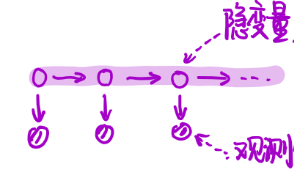
\includegraphics[width=.45\textwidth]{微信图片_20200107212223.png}
    \caption{Dynamic Model拓扑结构图}
    \label{fig:my_label_1}
\end{figure}

Dynamic Model可以从两个层面来看,横着看就是time的角度,如果是竖着看就可以表达为$P(X|Z)$的形式,也就是Mixture的形式。概率系统根据状态与状态之间的关系,可以分为两类。

如果是离散的则有HMM算法。

如果是连续的,按照线性和非线性可以分为Kalman Filter和Paricle Filter。

\section{HMM算法简介}
Hidden Markov Model的拓扑结构图如下所示:
\begin{figure}[H]
    \centering
    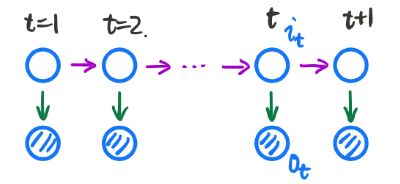
\includegraphics[width=.45\textwidth]{微信图片_20200107213811.png}
    \caption{Hidden Markov Model拓扑结构图}
    \label{fig:my_label_1}
\end{figure}

大家看到这个模型就会觉得和上一讲提到的,MCMC模型方法有点类似。HMM可以看做一个三元组$\lambda = (\pi, \mathcal{A}, \mathcal{B})$。其中:

$\pi$:是初始概率分布。

$\mathcal{A}$:状态转移矩阵。

$\mathcal{B}$:发射矩阵。

拓扑结构图的第二行为观测变量,观测变量$o$:$o_1,o_2,\cdots,o_t,\cdots \leftarrow \mathcal{V} = {v_1,v_2,\cdots,v_M}$。其中$\mathcal{V}$是观察变量$o$的值域,代表每一个观测变量$o_i$可能有$M$个状态。

拓扑结构图的第一行为状态变量,状态变量$i$:$i_1,i_2,\cdots,i_t,\cdots \leftarrow \mathcal{Q} = {q_1,q_2,\cdots,q_N}$。其中$\mathcal{Q}$是状态变量$i$的值域,代表每一个状态变量$i$可能有$N$个状态。

$\mathcal{A} = [a_{ij}]$表示状态转移矩阵,$a_{ij} = P(i_{i+1}=q_j|i_t=q_i)$。

$\mathcal{B} = [b_j(k)]$表示发射矩阵,$b_j(k) = P(o_t = V_k | i_t = q_j)$。

而$\pi$是什么意思呢?假设当$t$时刻的隐变量$i_t$,可能有$\{ q_1,q_2,\cdots,q_N \}$个状态,而这些状态出现的概率分别为$\{ p_1,p_2,\cdots,p_N \}$。这就是一个关于$i_t$隐变量的离散随机分布。

$\mathcal{A}$表示为各个状态转移之间的概率。

$\mathcal{B}$表示为观测变量和隐变量之间的关系。

\subsection{两个假设}
这是有关Hidden Markov Model的两个假设:

1. 齐次Markov假设(无后向性);2. 观察独立假设。

\textbf{齐次马尔可夫假设:}未来与过去无关,只依赖与当前的状态。也就是:
\begin{equation}
    P(i_{t+1}|i_{t},i_{t-1},\cdots,i_1,o_t,\cdots,o_1) = P(i_{t+1}|i_t)
\end{equation}

2. \textbf{观测独立假设:}
\begin{equation}
    P(o_{t}|i_{t},i_{t-1},\cdots,i_1,o_t,\cdots,o_1) = P(o_{t}|i_t)
\end{equation}

\subsection{三个问题}
1. Evaluation的问题,我们要求的问题就是$P(O|\lambda)$。也就是前向后向算法,给定一个模型$\lambda$,求出观测变量的概率分布。

2. Learning的问题,$\lambda$如何求的问题。也就是$\lambda_{MLE} = \arg\max_{\lambda}P(O|\lambda)$。求解的方法是EM算法和Baum Welch算法。

3. Decoding的问题,状态序列为$I$,也就是隐变量序列,$\hat{I} = \arg\max_{I}P(I|O,\lambda)$。也就是在在观测变量$O$和$\lambda$的情况下使隐变量序列$I$出现的概率最大。而这个问题大致被分为预测和滤波。

预测问题为:$P(i_{t+1}|o_1,\cdots,o_t)$;也就是在已知当前观测变量的情况下预测下一个状态,也就是Viterbi算法。

滤波问题为:$P(i_{t}|o_1,\cdots,o_t)$;也就是求$t$时刻的隐变量。

~\\

Hidden Markov Model,可以被我们总结成一个模型$\lambda = (\pi,\mathcal{A},\mathcal{B})$,两个假设,三个问题。而其中我们关注得最多的就是Decoding的问题。

\end{document}